% Intended LaTeX compiler: xelatex
\documentclass{orgstandard}
\author{Sebastian Meisel}
\date{\today}
\title{Zusammenfassung zum Thema DORA-Metriken\\\medskip
\large ITIL}
\hypersetup{
 pdfauthor={Sebastian Meisel},
 pdftitle={Zusammenfassung zum Thema DORA-Metriken},
 pdfkeywords={},
 pdfsubject={},
 pdfcreator={Emacs 29.1 (Org mode 9.6.6)}, 
 pdflang={German}}
\begin{document}

\maketitle


\section{DORA-Metriken in DevOps}
\label{sec:org8364cba}
\begin{itemize}
\item DORA steht für "DevOps Research and Assessment".
\item Ursprünglich entwickelt, um die Leistung von Softwareteams zu messen und zu verbessern.
\item Sie sind das Ergebnis umfangreicher Forschung und Analyse.
\end{itemize}

\subsection{Deployment-Frequenz}
\label{sec:org26a6802}
\begin{itemize}
\item Wie oft wird Software in die Produktion oder in einen produktionsähnlichen Zustand freigegeben?
\item Einfach ausgedrückt: Wie oft schickt das Team neue Software an die Kunden?
\end{itemize}
\begin{figure}[htbp]
\centering
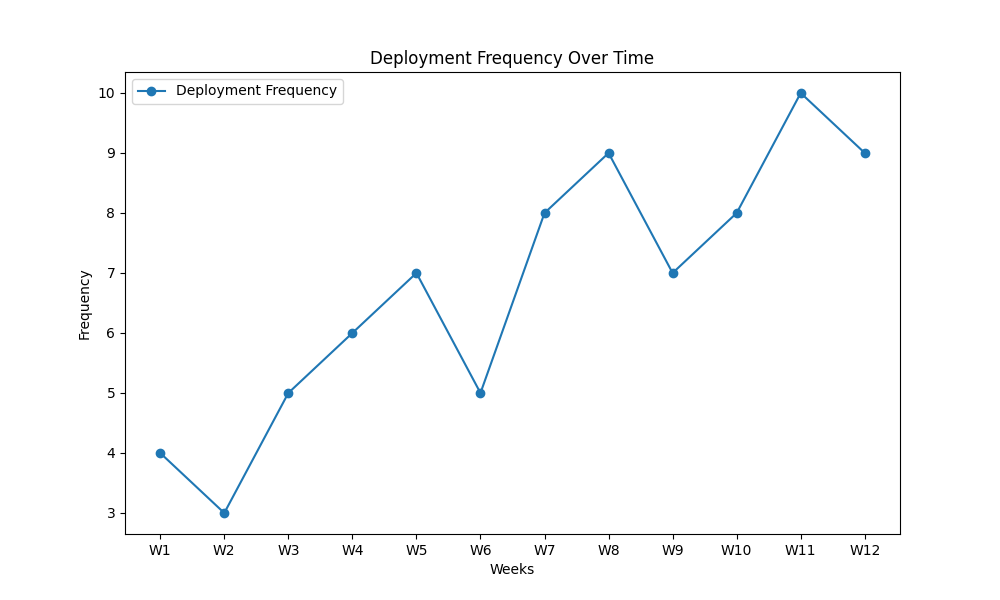
\includegraphics[width=.65\linewidth]{img/DeploymentFrequency.png}
\caption{\label{fig:orge492662}Deployment-Frequenz}
\end{figure}

\subsection{Lead-Time für Änderungen}
\label{sec:orgc80756c}
\begin{itemize}
\item Wie lange dauert es, eine Codeänderung von der Commit-Phase bis zur Produktion zu bringen?
\item Wie lange dauert es, bis eine neue Idee oder Fehlerbehebung beim Kunden ankommt?
\end{itemize}
\begin{figure}[htbp]
\centering
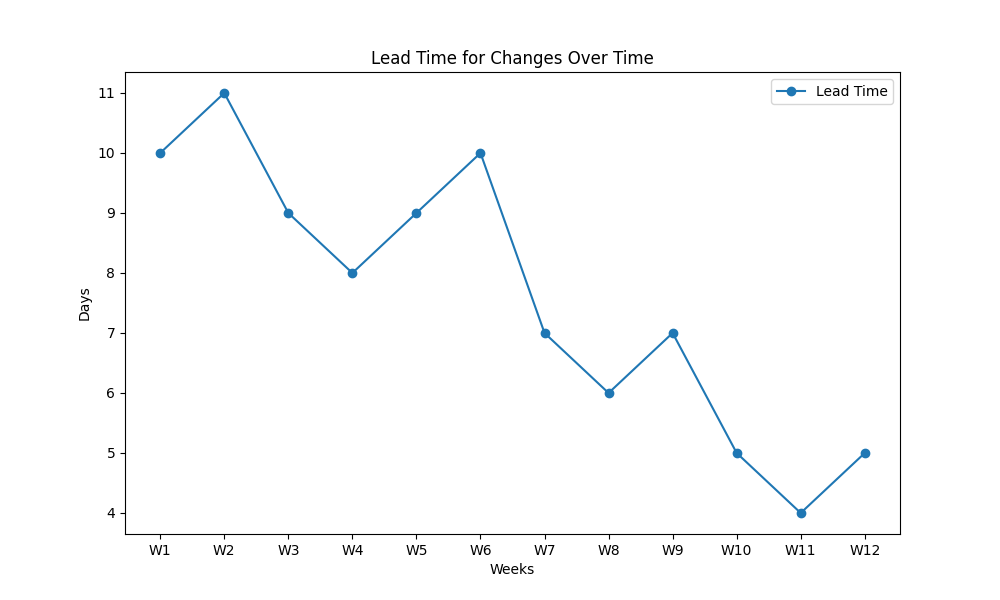
\includegraphics[width=.65\linewidth]{img/LeadTimeForChanges.png}
\caption{\label{fig:org3dc4154}Lead Time for Changes}
\end{figure}

\subsection{Mean Time to Restore (MTTR)}
\label{sec:org95d3489}
\begin{itemize}
\item Wie schnell können Sie von einem Ausfall oder einem anderen unerwünschten Ereignis erholen?
\item Wie schnell ist das Team, wenn etwas schiefgeht, um es wieder in Ordnung zu bringen?
\end{itemize}
\begin{figure}[htbp]
\centering
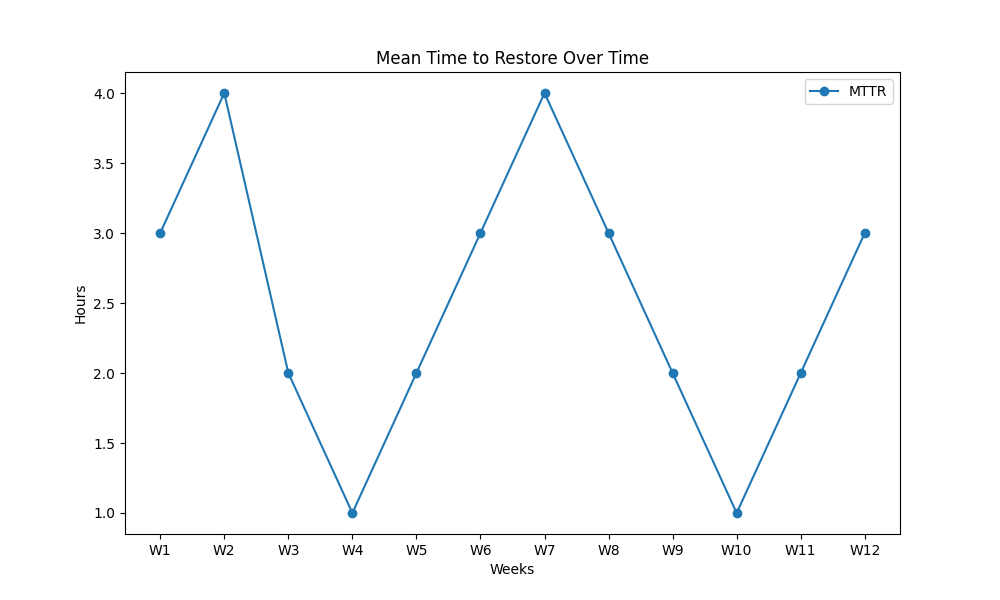
\includegraphics[width=.65\linewidth]{img/MTTR.png}
\caption{\label{fig:org414b74a}Mean Time to Restore}
\end{figure}

\subsection{Change Failure Rate}
\label{sec:org7c5ee15}
\begin{itemize}
\item Wie oft führen Änderungen zu einem Ausfall oder einer Beeinträchtigung des Dienstes?
\item Wie oft geht etwas schief, wenn neue Software veröffentlicht wird?
\end{itemize}
\begin{figure}[htbp]
\centering
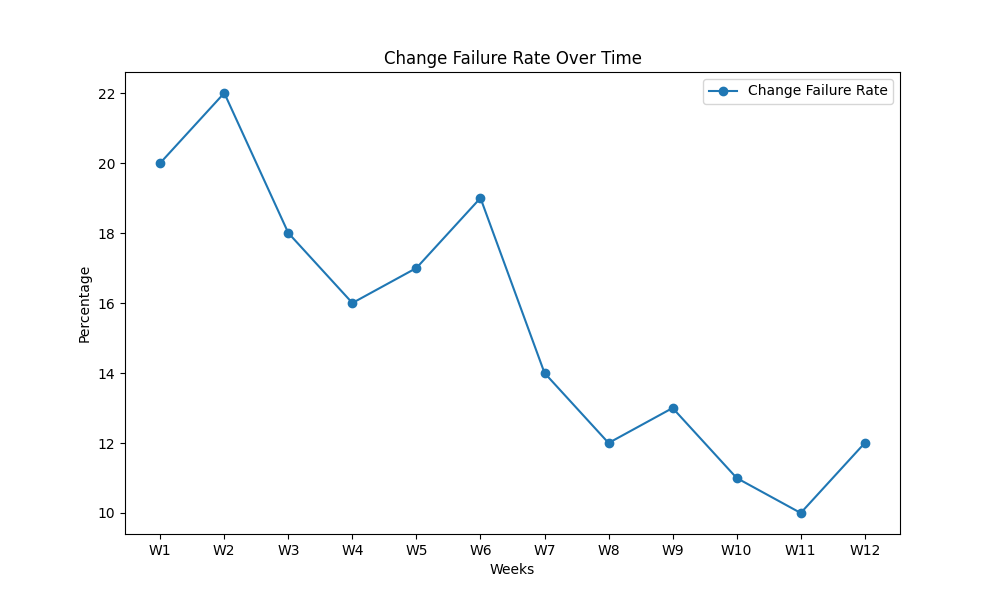
\includegraphics[width=.65\linewidth]{img/ChangeFailureRate.png}
\caption{\label{fig:org2c1d94b}Change Failure Rate}
\end{figure}

\section{Bedeutung der DORA-Metriken}
\label{sec:orgf74cefb}
\begin{itemize}
\item Diese Metriken bieten einen objektiven Überblick über die Leistungsfähigkeit des Entwicklungsprozesses.
\item Sie helfen, Engpässe zu identifizieren und Verbesserungsmöglichkeiten zu erkennen.
\end{itemize}

\section{Vergleich zu anderen Ansätzen}
\label{sec:orged69077}
\begin{itemize}
\item \textbf{Velocity in Agile}
\begin{itemize}
\item Misst, wie viel Arbeit ein Team in einem bestimmten Zeitraum erledigen kann.
\end{itemize}
\item \textbf{Bug Rate}
\begin{itemize}
\item Die Anzahl der Fehler, die in einem bestimmten Zeitraum gemeldet werden.
\end{itemize}
\item \textbf{Code Churn}
\begin{itemize}
\item Wie oft der Code geändert wird, kann auf instabile Bereiche hinweisen.
\end{itemize}
\item \textbf{Customer Satisfaction}
\begin{itemize}
\item Direktes Feedback von den Endbenutzern über die Qualität der Software.
\end{itemize}
\end{itemize}

\section{Unterschiede und Gemeinsamkeiten}
\label{sec:org3cae60d}
\begin{itemize}
\item \textbf{DORA} fokussiert auf den gesamten Entwicklungszyklus, während andere Metriken oft nur Teilaspekte abdecken.
\item \textbf{DORA}-Metriken sind oft einfacher zu messen und zu interpretieren.
\item Andere Metriken können subjektiver sein oder mehr Interpretation erfordern.
\end{itemize}
\end{document}